%!TEX root = ../dokumentation.tex

\section{Überarbeitete Systemarchitektur}

Im Konzept wurde bereits ein Kommunikationsablauf\footnote{Konzeptkapitel 4.1 Seite 28} konstruiert. Aufgrund der weiteren Recherche zum Thema Google Cloud Messaging und dem erfolgreichen Abschluss der Proof-of-Concepts, konnte die angedachte Systemarchitektur überarbeitet werden.

Der Kommunikationsablauf ging davon aus, dass kein Rückkanal bei Google Cloud Messaging verfügbar ist. Auf Grund dieser Annahme wurde neben GCM eine weitere Schnittstelle eingeplant, welche auf dem REST Paradigma basierte. Die dadurch nur mögliche synchrone Interaktion ist jedoch eine großer Nachteil für die geplanten Features gewesen. Außerdem kann die Wartung von zwei Architekturen auf längere Zeit zu Problemem führen.\\

Durch die bidirektionale Verbindung zwischen Client und Server bzw Server und Client kann der Google Dienst „GCM Cloud Connection Server“ die aufgeführte Problematik lösen.

In der neuen Systemarchitektur (vgl Abb. \ref{fg:gcmccsarchitecture}) ist die REST Schnittstelle entfernt worden und jedes Endgerät hat einen Rückkanal zu den GCM Connection Servern bekommen. Auch unser Serverinfrastruktur hat nun einen direkten Zugriff über eine XMPP Verbindung zu dem GCM Endpoint. Hierbei werden die die Daten im JSON Format in einem XMPP Paket verschickt.

Die Serverdatenbank wird auf dem MySQL Datenbanksystem aufgebaut (siehe hierzu auch Kapitel „Entwickeltes System“). Als weitere Ergänzung gegeüber dem Konzept ist der Message Broker, welcher die verschiedenen Nachrichtentypen an den zugehörigen Controller - optional gebündelt - weiterleitet.

\begin{figure}[H]
	\centering
	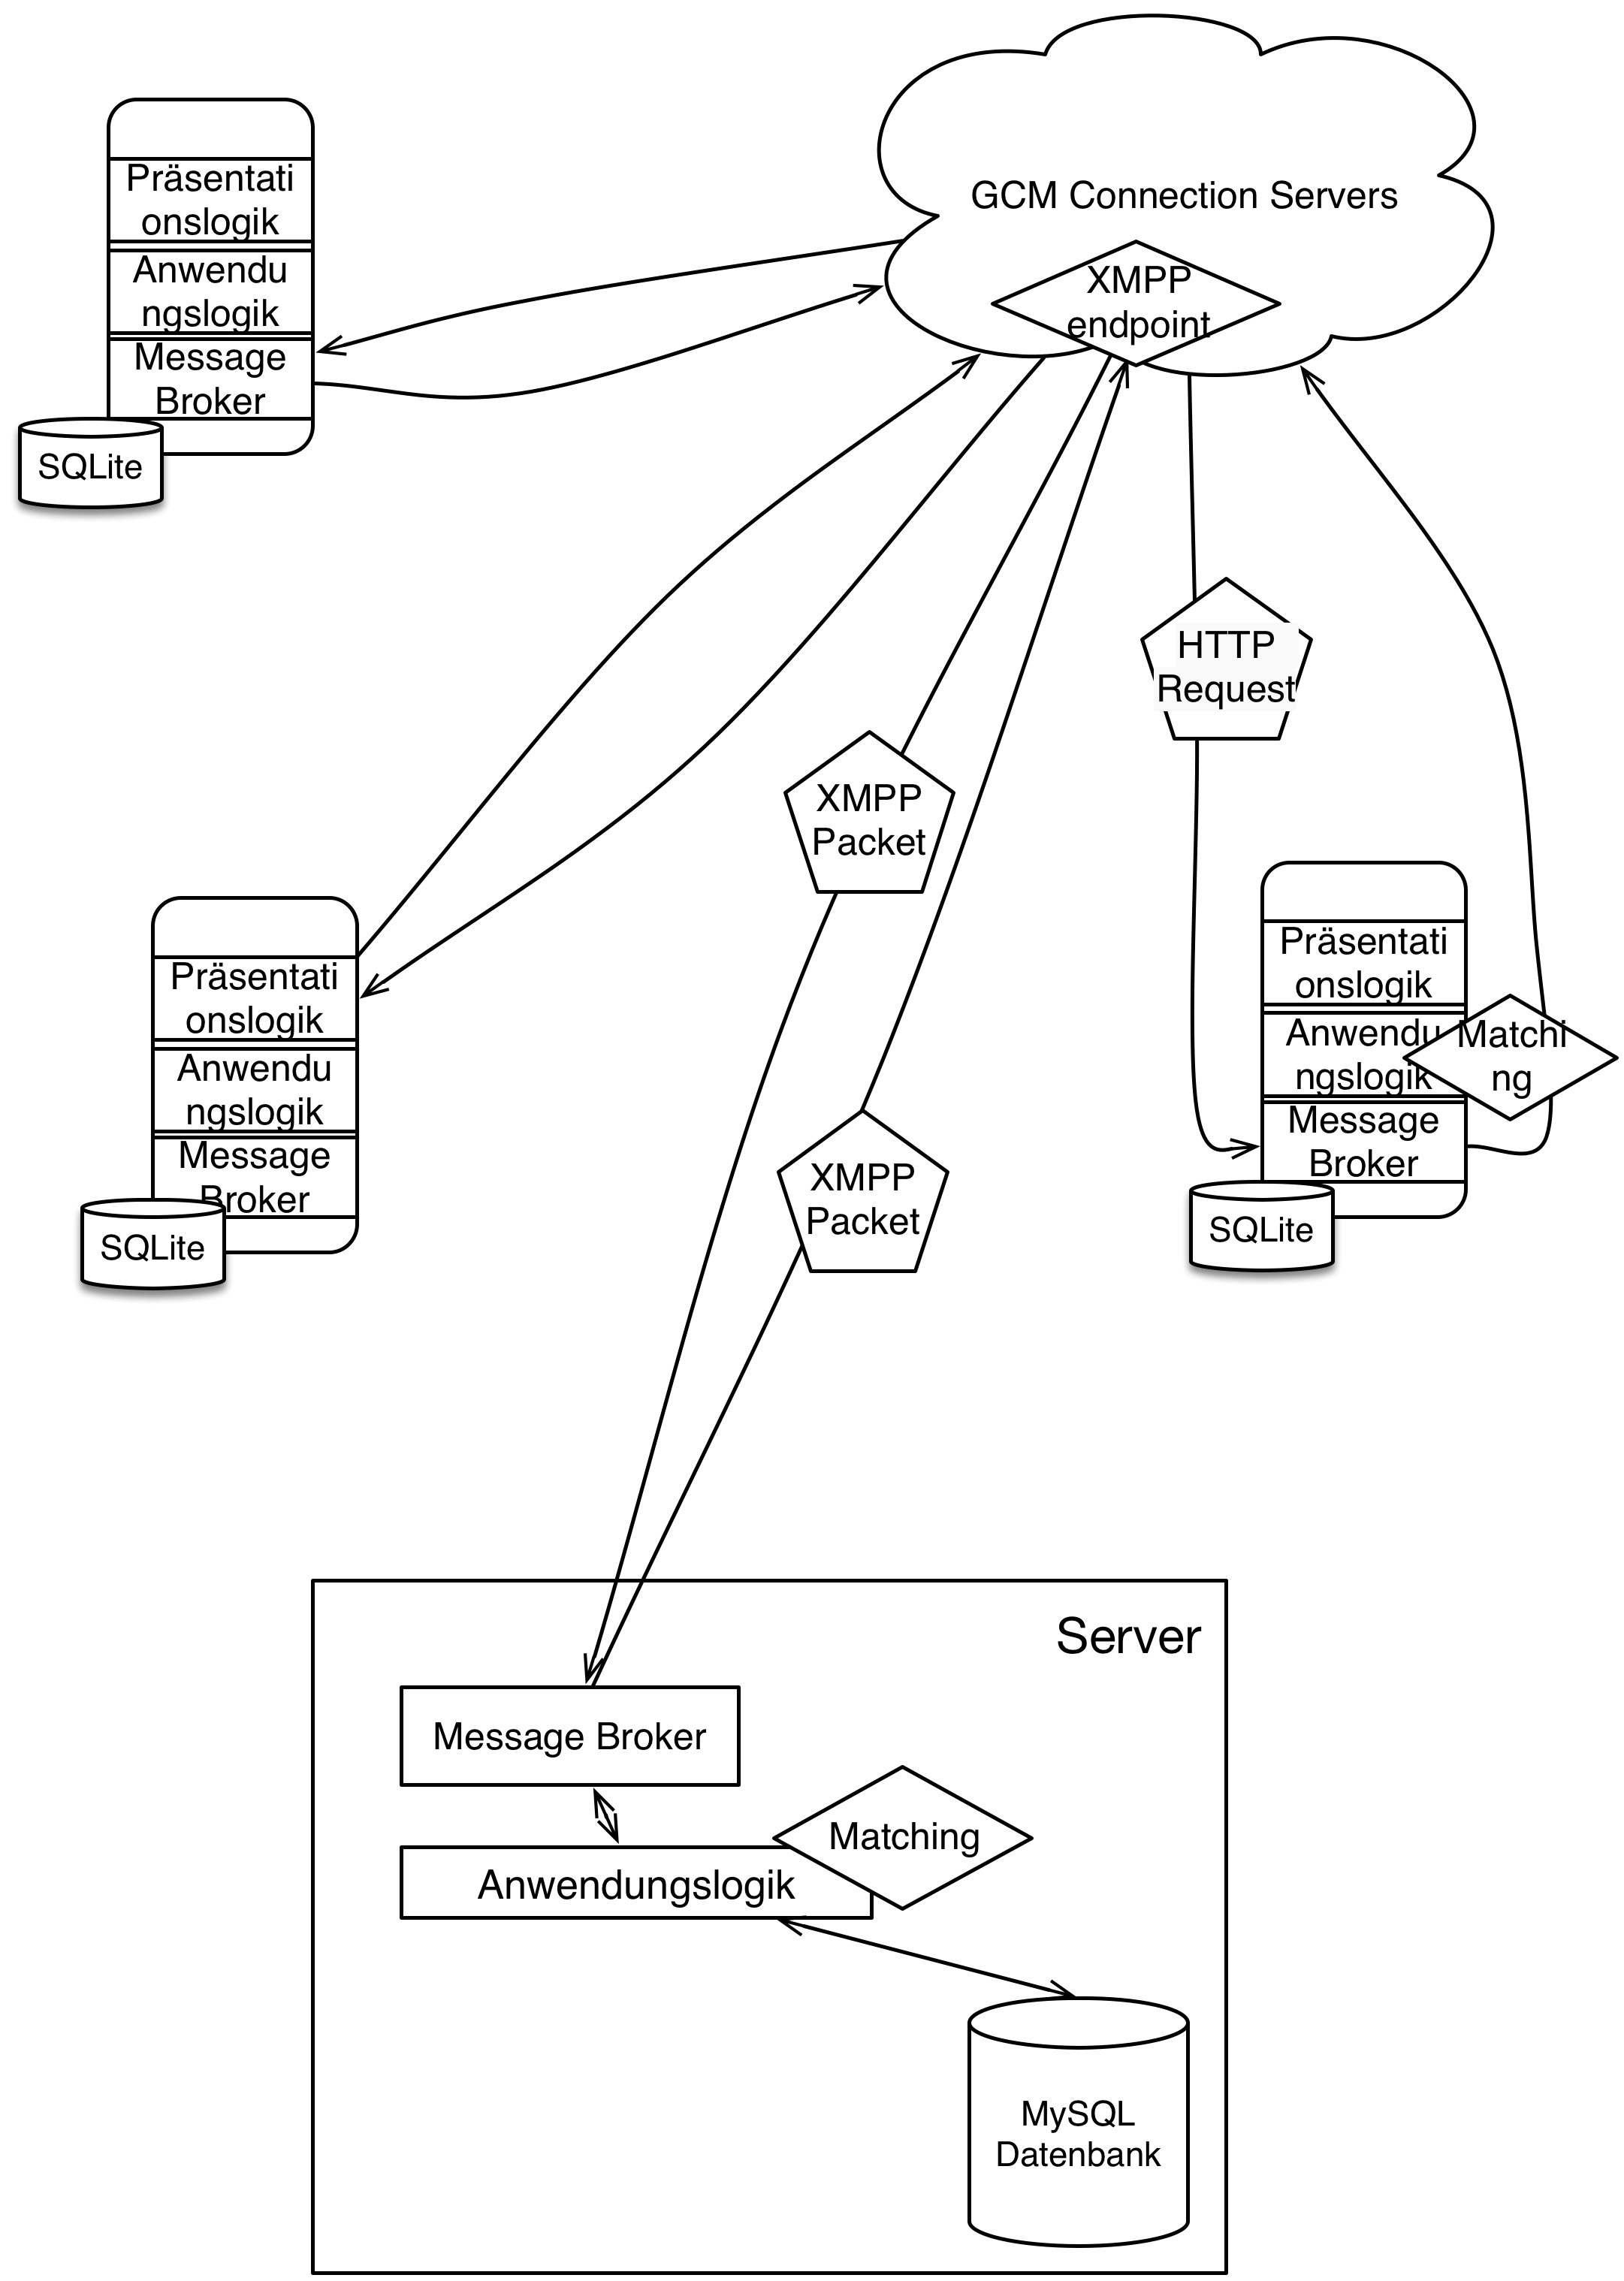
\includegraphics[width=0.85\textwidth]{./images/architekturneu.png}
	\caption{Systemarchitekur mit „GCM Cloud Connection Server“}
	\label{fg:gcmccsarchitecture}
\end{figure}
